\documentclass[11pt]{beamer}
\usepackage[utf8]{inputenc}
\usepackage[german]{babel}
\usepackage[T1]{fontenc}
\usepackage{xcolor}
%\usepackage[usefilenames, RMstyle=Light, SSstyle=Light, TTstyle=Light, DefaultFeatures={Ligatures=Common}]{plex-otf} 
\usepackage{amsmath}
\usepackage{amsfonts}
\usepackage{amssymb}
\usepackage{graphicx}
\usepackage{csquotes}
\usetheme{Dresden}
\author{Felix Beckmann, Leonhard Alkewitz, Max Lautenbach}
\title{Die Optimierung der Energiebilanz von simulierten Gebäuden mit Hilfe von evolutionären Algorithmen}
%\setbeamercovered{transparent} 
%\setbeamertemplate{navigation symbols}{} 
\logo{
\includegraphics[scale=.05]{logo.png}} 
\institute{Spezialschulteil des Albert-Schweizer Gymnasium Erfurt} 
\date{\today} 
%\subject{} 

\begin{document}

\begin{frame}
\begin{center}
\pause \huge{2 376 000 000 000 000 $J$}  \\  
\pause \huge{641 000 000 $kWh$} \\ 
\pause \huge{81 000 000 $kg$ $SKE$ \footnote{SKE = Steinkohleeinheit}} \\ 
\hrulefill{}  \\
\pause \huge{2000-2500 $l$} \\ 
\pause \huge{10-15 $Badewannen$}
\end{center}
\end{frame}

\begin{frame}
\titlepage
\end{frame}

\begin{frame}
\begin{enumerate}
\item{Einführung in die Thematik der Optimierung und der Energiebilanz von Gebäuden}
\begin{enumerate}
\item{Verfahren zur evolutionären Optimierung}
\item{Ermittlung der Energiebilanz von Gebäuden}
\end{enumerate}
\item{Zielstellung der Seminarfacharbeit und Abgrenzung des Themas}
\item{Methodik zum Erreichen unserer Ziele und Vorstellung des Zeitplans}
\item{Motivation und Begründung zur Wahl dieses Themas}
\end{enumerate}
\end{frame}

\begin{frame}{Einführung in die Thematik der Optimierung und der Energiebilanz von Gebäuden}
\framesubtitle{\large{\textcolor{black}{Verfahren zur evolutionären Optimierung}}}
\begin{figure}
\includegraphics[scale=0.12]{Scan9}
\caption{Modell der Evolution}
\end{figure}
\end{frame}

\begin{frame}{Einführung in die Thematik der Optimierung und der Energiebilanz von Gebäuden}
\framesubtitle{\large{\textcolor{black}{Ermittlung der Energiebilanz von Gebäuden}}}
\begin{figure}
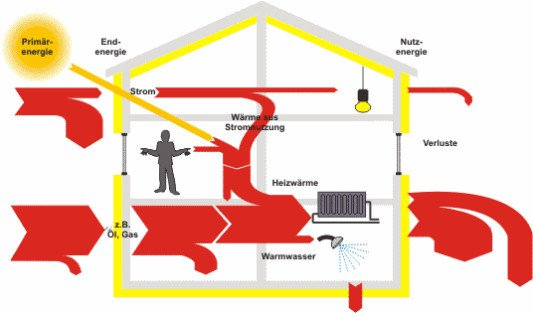
\includegraphics[scale=0.45]{0dd5dc31023435ef-2.jpg} 
\caption{Erstellen der Energiebilanz}
\end{figure}
\end{frame}

\begin{frame}{Motivation und Begründung zur Wahl dieses Themas}
\begin{itemize}
\pause
\item{hohes Potential die Energiebilanz von Wohngebäuden zu verbessern}\pause
\item{Affinität zur Informatik, Architektur und Bauphysik}\pause
\item{Verbinden von Informatik und Physik in Form von Algorithmen und Bauphysik}\pause
\item{Anwenden von evolutionären Algorithmen auf ein reales Problem}\pause
\item{automatisierte Planung von Häusern unter Einbezug von Energiebilanz und Statik}\pause
\item{entdecken möglicher unkonventioneller Hausformen}
\end{itemize}
\end{frame}
\begin{frame}
\begin{thebibliography}{9}
\bibitem{1}
\textcolor{black}{\url{https://www.bmwi.de/Redaktion/DE/Downloads/Energiedaten/energiedaten-gesamt-pdf-grafiken.pdf?__blob=publicationFile&v=38}; zuletzt besucht: 26.09.2018}
\bibitem{2}
\textcolor{black}{
\url{https://ag-energiebilanzen.de/index.php?article_id=29&fileName=ausw_30jul2018_ov.pdf}; zuletzt besucht: 26.09.2018}
\end{thebibliography}
\end{frame}
\begin{frame}{Bildquellen}
\begin{thebibliography}{9}
\bibitem{1}
\textcolor{black}{
\textit{Abbildung 1}; Prof. Dr. Jürgen Markl, Markl Biologie; S. 256.1; 1. Auflage; Ernst Klett Verlag, Stuttgart, 2010}
\bibitem{2}
\textcolor{black}{
\textit{Abbildung 2}; \url{https://www.baunetzwissen.de/imgs/5/7/5/8/5/3/0dd5dc31023435ef.jpg}; zuletzt besucht: 27.09.2018}
\end{thebibliography}
\end{frame}
\end{document}